\begin{Exercise}[title=Catapulte de porte-avions]
Une catapulte à avions est montée sur un navire militaire). Elle est constituée d’un réservoir de vapeur connecté à un long cylindre, dans lequel glisse un piston entraînant l’avion au décollage.
  \centering
  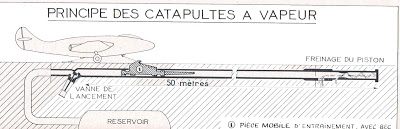
\includegraphics[width=0.4\textwidth]{catapulte.jpg}

	Au début du catapultage, la vapeur est à~\SI{140}{\bar} et~\SI{700}{\degreeCelsius}. Après une brève course de~\SI{50}{\metre}, l’avion a quitté le pont et la vapeur est à~\SI{4}{\bar} et~\SI{410}{\degreeCelsius}.


		\Question Quelle énergie la catapulte a-t-elle fourni à l’avion par kilo de vapeur ?
		\Question Quelles doivent être le diamètre du piston et la masse totale de vapeur, pour que la poussée fournie à l’avion soit toujours supérieure à~\SI{2,5}{\tonne} ?

\end{Exercise}
\begin{Answer}
  \Question $\Delta u = \SI{-433,1}{\kilo\joule\per\kilogram}$ ($=w_\fromatob$ si l’on suppose l’évolution adiabatique) ;
\Question $D_\text{min.} = \SI{32,26}{\centi\metre}$ (attention à tenir compte de la
pression atmosphérique) ;
$m = \frac{V_\text{max} - V_\text{min}}{v_\text{max} - v_\text{min}} = \SI{5,243}{\kilogram}$.
NB: faute de sources fiables, les données de cet exercice sont purement imaginaires.
\end{Answer}
